% Effect of line-of-sight context on the 2-D slice rhizome.
% Numbers: CompAstro wiki, "Rhizome Neural Operator Results" §2 (sweep, 15k steps, one seed).
\documentclass[border=4pt]{standalone}
\usepackage[T1]{fontenc}
\IfFileExists{fourier.sty}{\usepackage{fourier}}{\usepackage{lmodern}}
\usepackage{amsmath}
\usepackage[dvipsnames]{xcolor}
\usepackage{pgfplots}
\pgfplotsset{compat=1.16}
\begin{document}
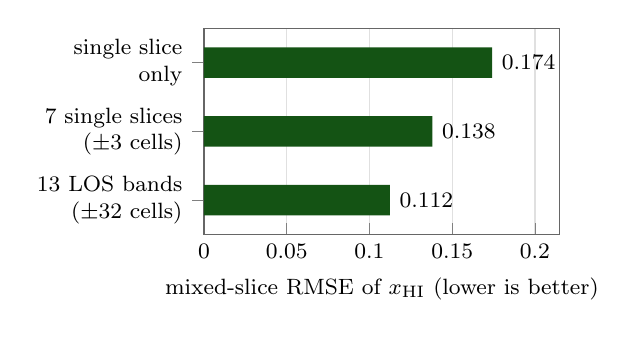
\begin{tikzpicture}
\begin{axis}[
    xbar, bar width=11pt,
    width=6.1cm, height=4.2cm,
    xmin=0, xmax=0.215, xtick={0,0.05,0.1,0.15,0.2},
    xlabel={mixed-slice RMSE of $x_{\mathrm{HI}}$ (lower is better)},
    xlabel style={font=\footnotesize},
    symbolic y coords={all,singles,center},
    ytick=data,
    yticklabels={{13 LOS bands\\($\pm32$ cells)},{7 single slices\\($\pm3$ cells)},{single slice\\only}},
    yticklabel style={font=\footnotesize, align=right},
    tick label style={font=\footnotesize},
    enlarge y limits=0.25,
    xmajorgrids, grid style={black!12},
    scaled x ticks=false, xticklabel style={/pgf/number format/fixed, /pgf/number format/precision=2},
    nodes near coords, nodes near coords style={font=\footnotesize, anchor=west},
    point meta=explicit symbolic,
    axis line style={black!60},
    ytick pos=left, xtick pos=bottom,
  ]
  \addplot[fill=ForestGreen!60!black, draw=none] coordinates {
    (0.1123,all) [0.112] (0.1380,singles) [0.138] (0.1741,center) [0.174]};
\end{axis}
\end{tikzpicture}
\end{document}
